\documentclass{beamer}

\usetheme{Boadilla}
\setbeamertemplate{frametitle}[default][center]
\setbeamertemplate{bibliography item}[text]

% --- Packages ---
\usepackage{graphicx}
\usepackage{booktabs}
\usepackage{siunitx}
\usepackage{tabularx}
\usepackage{xcolor}
\usepackage[thinc]{esdiff}




\usepackage{amsmath}
\usepackage{ gensymb }
\usepackage{caption}
\usepackage{subcaption}
\usepackage{hyperref} 

% --- Bibliography ---
\bibliographystyle{apalike}

\newcommand{\backupbegin}{
   \newcounter{finalframe}
   \setcounter{finalframe}{\value{framenumber}}
}
\newcommand{\backupend}{
   \setcounter{framenumber}{\value{finalframe}}
}


\setbeamertemplate{frametitle}[default][center]
\usefonttheme{professionalfonts}
\setbeamertemplate{navigation symbols}{}

\subtitle{Climate dynamics department meeting}
\title{The impact of tropospheric versus stratospheric CO$_2$ forcing on the Hadley cell }
%\titlegraphic{\includegraphics[width=0.9\linewidth,height=0.4\linewidth]{image.png}}
%\author{Ole Merkes}
\author[Ole Merkes]{Ole Merkes \\[1\baselineskip]
Supervised by Sarah Kang and Moritz Günther \\
}
%\institute{University of Hamburg, Max-Planck-Institute for Meteorology}
\date{\today}
\titlegraphic{%
  \makebox[0.95\paperwidth]{%
    
\includegraphics[height=1cm,keepaspectratio]{figures/mpi_logo.png}%
    \hspace{6cm}%
    
\includegraphics[height=1.5cm,keepaspectratio]{figures/uhh-logo.pdf}%
  }%
}
% \titlegraphic{
\includegraphics[height=1cm,keepaspectratio]{figures/mpi_logo.png}\hfill
%    
\includegraphics[height=1cm,keepaspectratio]{figures/uhh-logo.pdf}
% }


\AtBeginSection[]
{
    \begin{frame}
        %\frametitle{Table of Contents}
        \tableofcontents[currentsection,currentsubsection]
    \end{frame}
}

\begin{document}

% \setbeamertemplate{background canvas}{
% \transparent{0.4}\includegraphics[width=\paperwidth,height=\paperheight]{image.png}
% }%
\begin{frame}
    \titlepage
\end{frame}
%\setbeamertemplate{background canvas}[default]
\section{Introduction}

\begin{frame}
    \frametitle{The Hadely cell (HC) under greenhouse gas forcing}
    \begin{block}{Model intercomparison studies}
        \begin{itemize}
            \item HC \textbf{weakening} of 1.2\%/K \cite{Lu2007}
            \item HC \textbf{widening}  at the poleward edge of 0.7°/K \cite{DAgostino2017}
            \item Linked to changes in tropopheric depth, meridional temperature gradient, and vertical stability \cite{LionelloEtAl2024}
            %\item HC widening is larger in the SH, weakening larger in the NH \cite{LionelloEtAl2024} 
        \end{itemize}
        \centering
    \end{block}
    \vfill
    \textbf{Is this also true if we decompose the CO$_2$ forcing vertically.}
\end{frame}

\begin{frame}
    \frametitle{Model: ECHAM 6}
    \begin{itemize}
        \item CMIP6 type general circulation model
        \item Mixed-layer ocean ($d=50\;\unit{\m}$) configuration
        \item 47 vertical pressure levels with (lat,lon)$=(96,192)$ gridpoints ($\sim 200\;\unit{\km}$)
        \item 4 runs: pre-industrial, uniform 4xCO$_2$, 4xCO$_2$ troposphere, 4xCO$_2$ stratosphere
    \end{itemize}
\end{frame}

\begin{frame}
    \frametitle{Linear decomposition of forcing works}
    \begin{figure}
        \centering
        
\includegraphics[width=\textwidth]{figures/t_uniform.png}
    \end{figure}
\end{frame}

\begin{frame}
    \frametitle{Temperature anomalies}
    \begin{figure}
        \centering
        
\includegraphics[width=\textwidth]{figures/temperature.png}
    \end{figure}
\end{frame}

\begin{frame}
    \frametitle{Temperature anomalies}
    \begin{figure}
        \centering
        
\includegraphics[width=0.6\textwidth]{figures/temperature.png}
    \end{figure}
    \begin{block}{Yet to be clarified}
    \begin{itemize}
        \item Stratospheric cooling in 4xCO$_2$ Tropo
        \item Stratospheric warming in 4xCO$_2$ Strato
        \item one-dimensional RCE model \textit{konrad}
    \end{itemize}
    \end{block}
\end{frame}






\begin{frame}
    \frametitle{Zonally averaged circulation}
    \begin{figure}
        \centering
        
\includegraphics[width=\textwidth]{figures/streamfunc.png} %TODO
    \end{figure}
\end{frame}

\begin{frame}
  \frametitle{Changes in Hadley circulation}
\begin{table}[]
    \centering
    \begin{tabular}{c|ccc}
         &Uniform & Tropo & Strato \\ \toprule
        $\Delta\psi_\mathrm{max, NH}$& $-1.6\%$ & \textbf{$3.4\%$}& $-8.7\%$\\
        $\Delta\psi_\mathrm{max, SH}$ & $-1.4\%$ & $5.6\%$ & $-5.7\%$\\ 
        $\Delta\Phi_\mathrm{H, NH}$  & $1.6\unit{\degree}$& $0.8\unit{\degree}$ &$0.8\unit{\degree}$\\
        $\Delta\Phi_\mathrm{H, SH}$  & $-1.6\unit{\degree}$& $-1.0\unit{\degree}$ &$-0.6\unit{\degree}$\\
    \end{tabular}
    \label{tab:placeholder}
\end{table}
\begin{block}{Surprise}
    \begin{itemize}
        \item HC is \textbf{weakening} with stratospheric CO$_2$
        \item HC is \textbf{strengthening} with tropospheric CO$_2$
    \end{itemize}
\end{block}
\end{frame}


\begin{frame}
    \frametitle{Thesis topic}
    \begin{alertblock}{Research gap}
        Why is the HC weakening with stratospheric CO$_2$ forcing but strengthening with tropospheric CO$_2$ forcing.
    \end{alertblock}
    \begin{block}{Thesis approach}
        Employ dynamical theories of the HC to explain this behavior.
    \end{block}
\end{frame}
% \begin{frame}
%     \frametitle{Hadley cell climatology}
%     \begin{figure}
%         \centering
%         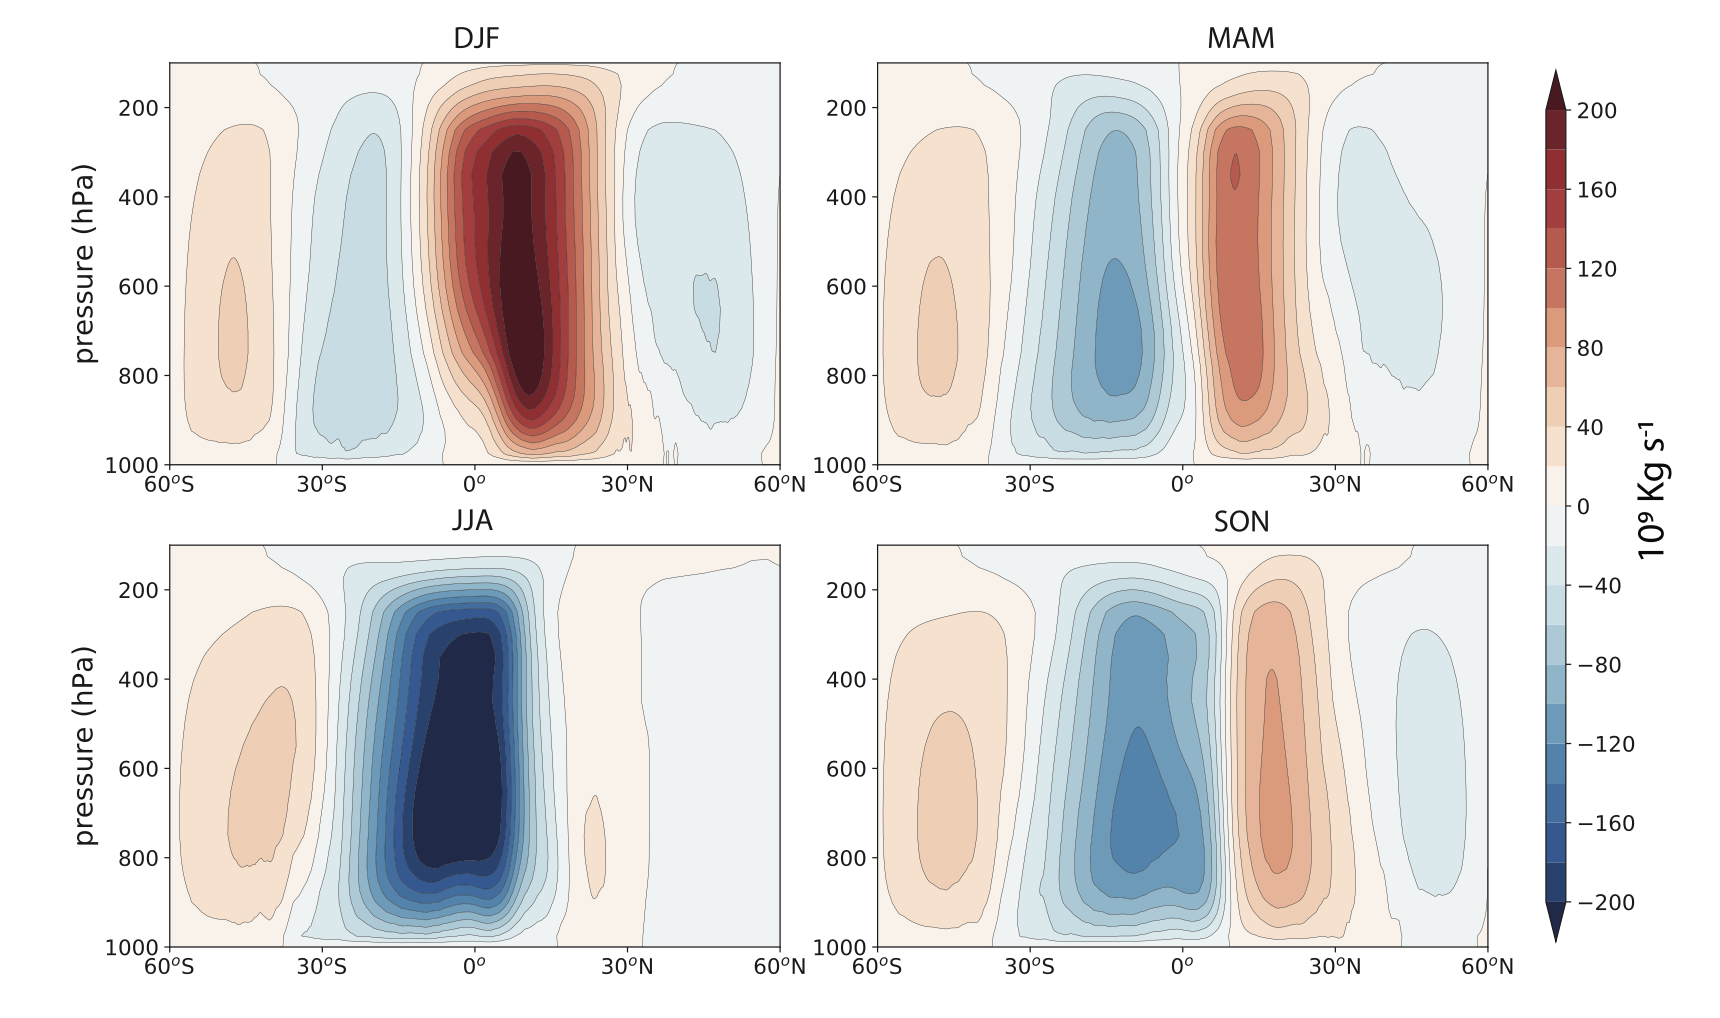
\includegraphics[width=\textwidth]{figures/HC_era5.png}
%         \caption{ERA5 data from 1979-2019 \cite{LionelloEtAl2024}.}
%     \end{figure}
% \end{frame}

% \begin{frame}
%     \frametitle{The HC is the dominant driver of tropical circulation}
%     \begin{block}{Significance}
%     \begin{itemize}
%         \item Ascending branch associated with \textbf{intense precipitation} 
%         \item Descending branch associated with the subtropical \textbf{dry} zones
%         \item Transports \textbf{energy} towards the poles and \textbf{moisture} to the equator
%         \item Closely tied to the \textbf{global monsoon} \cite{Bordoni2008} with more than 2 billion people affected
%     \end{itemize}
%     \end{block}
% \end{frame}

\section{Held\&Hou theory}

% \begin{frame}
%     \frametitle{The axisymmetric theory of the HC}
% \begin{figure}[t]
%      \centering
%      \begin{subfigure}[t]{0.47\textwidth}
%          \centering
%          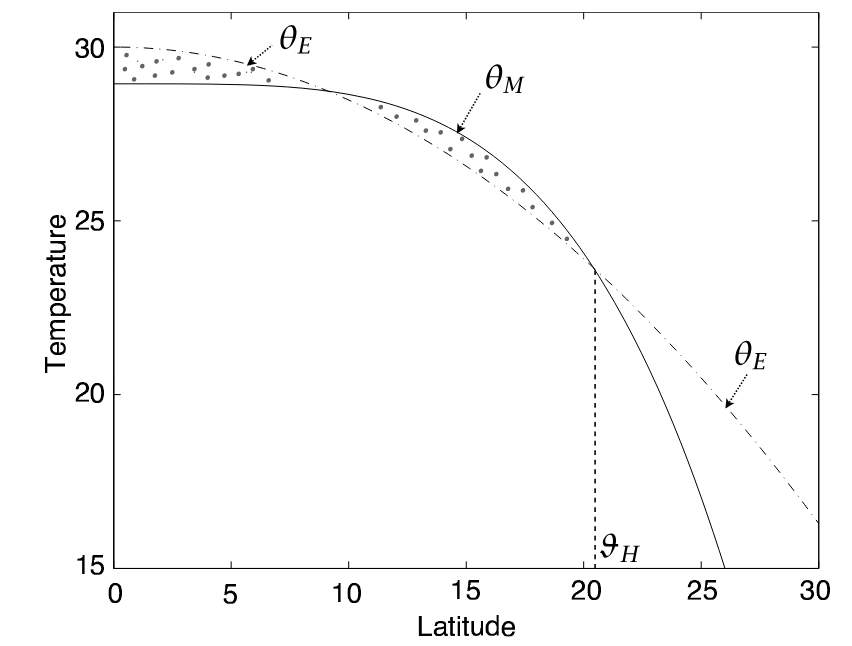
\includegraphics[width=\textwidth]{figures/temperature_vallis.png}
%          \label{fig:spread}
%      \end{subfigure}
%     \hspace{0.03\textwidth}
%      \begin{subfigure}[t]{0.47\textwidth}
%          \centering
%          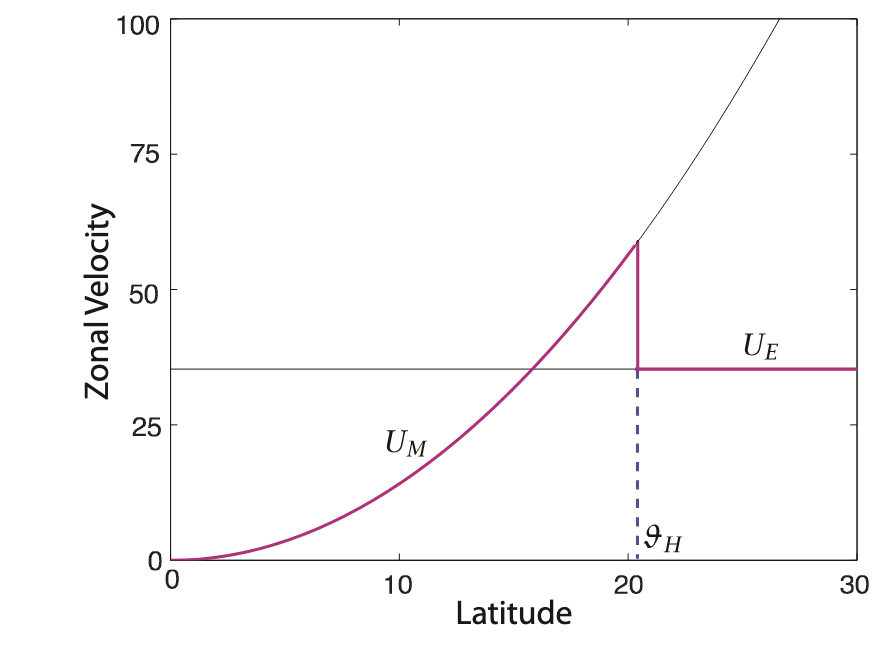
\includegraphics[width=\textwidth]{figures/zon_vel.png}
%      \end{subfigure}
%         \caption{Temperature und zonal velocities in the H\&H theory from \cite{Vallis2017}.}
%         \label{}
% \end{figure}
% \end{frame}

\begin{frame}
    \frametitle{The axisymmetric theory of the HC}
\begin{columns}
\begin{column}{0.5\textwidth}
    \begin{figure}
        \centering
        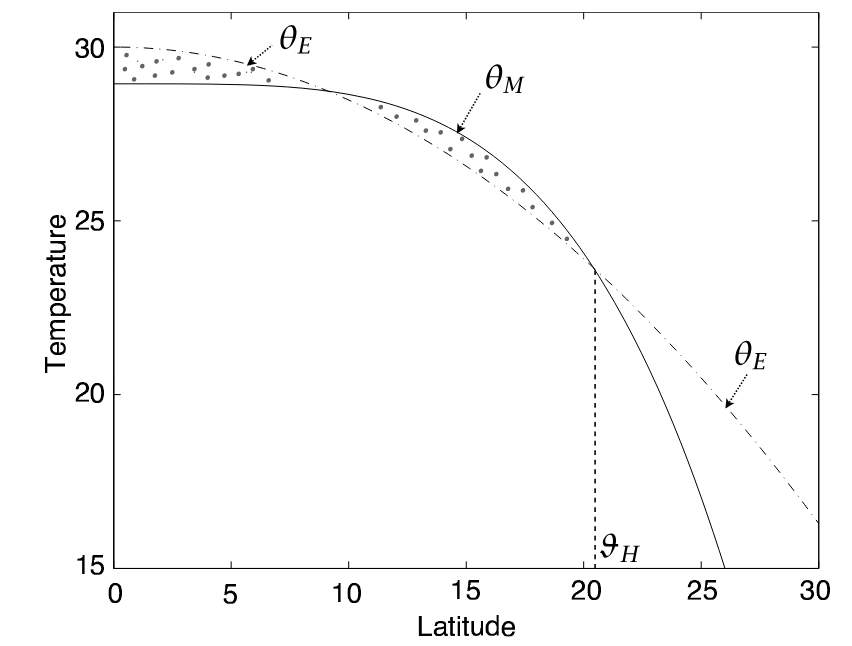
\includegraphics[width=\textwidth]{figures/temperature_vallis.png}
        \caption{The edge of the HC \cite{Vallis2017}.}
    \end{figure}
\end{column}
\begin{column}{0.45\textwidth}  %%<--- here
  \begin{block}{Width and extent of the HC \cite{HeldHou1980}}  
    \begin{align}
        \Phi_H\propto&\left(H\Delta_h\right)^{1/2}\\
        \psi_\mathrm{max} \propto & \frac{(H\Delta_h)^{5/2}}{\Delta_v}
    \end{align}
    \end{block}
    $H$: Troposphere depth\\
    $\Delta_h$: Fractional pole to equator temperature difference\\
    $\Delta_v$: Fractional surface to tropopause temperature difference
\end{column}
\end{columns}
\end{frame}

\begin{frame}
    \frametitle{Linearisation of direct thermodynamical drivers}
    \begin{align*}
        \frac{\delta\psi_\mathrm{max}}{\psi_\mathrm{max}}&=\frac{5}{2}\frac{\delta H}{H}+\frac{5}{2}\frac{\delta\Delta_h}{\Delta_h}-\frac{\delta\Delta_v}{\Delta_v}\\
        \frac{\delta\Phi_\mathrm{H}}{\Phi_\mathrm{H}}&=\frac{1}{2}\frac{\delta H}{H}+\frac{1}{2}\frac{\delta\Delta_h}{\Delta_h}
    \end{align*}
    \begin{itemize}
        \item meridional near-surface potential
        temperature contrast $\Delta_h=\Bar{\theta}(800-700\;\si{hPa},0-10\;\unit{\degree})-\Bar{\theta}(800-700\;\si{hPa},80-90\;\si{\degree})$
        \item subtropical static stability $\Delta_v=\Bar{\theta}(200\;\si{hPa},20-40\;\unit{\degree})-\Bar{\theta}(800\;\si{hPa},20-40\;\si{\degree})$
        \item tropical tropopause height $H=\Bar{H}(0-15\unit{\degree})$ 
    \end{itemize}
\end{frame}

\begin{frame}
    \frametitle{Does linearised H\&H explain the HC's response?}
    \begin{figure}
        \centering
        
\includegraphics[width=\textwidth]{figures/scatter_SH.png}
    \end{figure}
\end{frame}


\begin{frame}
    \frametitle{Why does H\&H fail to explain HC dynamics?}

    \begin{block}{Limitations}
        \begin{itemize}
            \item Idealized model without oceans, land mass, clouds, etc.
            \item Eddies and axially asymmetric flow
            \item Temperature scaling parameters are in radiative equilibrium 
        \end{itemize}
    \end{block}
\end{frame}

\section{Incorporating eddies}

\begin{frame}
    \frametitle{Indirect thermodynamical drivers}
\begin{columns}
\begin{column}{0.7\textwidth}
    % \begin{block}{Baroclinic instability}
    %     \begin{align}
    %         \Phi_H \sim& \left(\frac{NH}{2\Omega a}\right)^{1/2}
    %     \end{align}
    % \end{block}
    \begin{block}{Eddy momentum flux}
        \begin{equation}
            \psi(1-\mathrm{Ro})\approx \frac{S}{f}
        \end{equation}
        \begin{itemize}
            \item $\mathrm{Ro}\rightarrow 1$: Axisymmetric limit
            \item $\mathrm{Ro}\rightarrow 0$: Eddy momentum flux dominates
        \end{itemize}
    \end{block}
\end{column}
\begin{column}{0.25\textwidth}  %%<--- here
    % $H$: Troposphere depth\\
    % $N$: Brunt–Väisälä frequency\\
    $\mathrm{Ro}=\xi/f$: Local Rossby number \\
    $S$: Eddy momentum flux divergence
\end{column}
\end{columns}
\end{frame}

\begin{frame}
    \frametitle{Intermediate regimes}
    \begin{block}{Eddy momentum flux}
        \begin{equation*}
            \psi(1-\mathrm{Ro})\approx \frac{S}{f}
        \end{equation*}
        \begin{itemize}
            \item $\mathrm{Ro}\rightarrow 1$: Axisymmetric limit
            \item $\mathrm{Ro}\rightarrow 0$: Eddy momentum flux dominates
        \end{itemize}
    \end{block}

    \begin{alertblock}{$0<\mathrm{Ro}<1$}
        \textit{There is no theory that captures how the Hadley circulation responds to climate
changes in this intermediate range of Rossby numbers.} - \cite{LevineSchneider2011}
        
    \end{alertblock}

\end{frame}

\begin{frame}
    \frametitle{Annual mean and equinox HC are similar}
    \begin{figure}
        \centering
        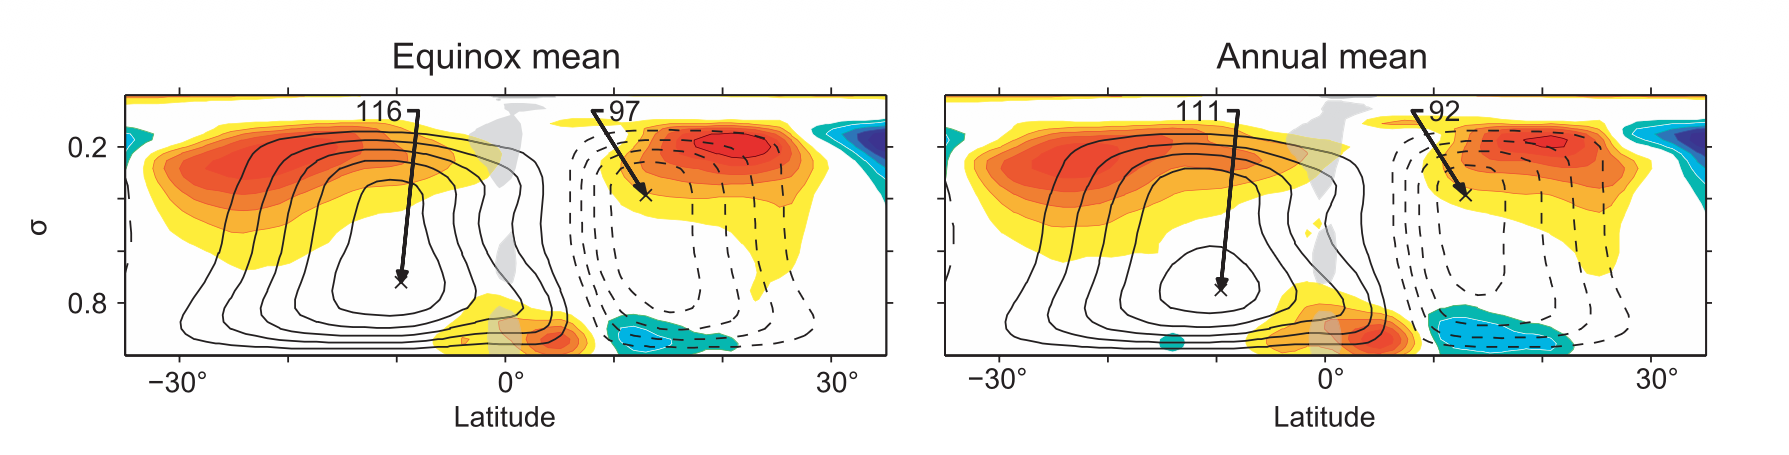
\includegraphics[width=\textwidth]{figures/ann_mean_equinox.png}
        \caption{Local Rossby numbers in equinox and annual mean case using reanalysis data from \cite{LevineSchneider2011}.}
    \end{figure}
\end{frame}

\begin{frame}
    \frametitle{HC strength and eddy momentum fluxes}
    \begin{figure}
        \centering
        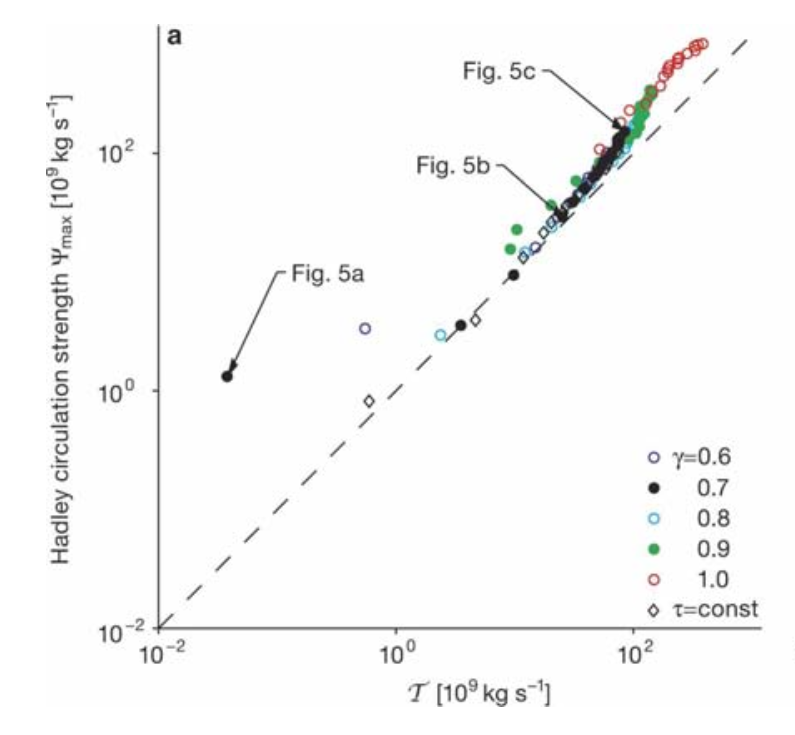
\includegraphics[height=0.7\textheight]{figures/eddy_strength.png}
        \caption{Linear relation between eddy momentum flux and HC strength from \cite{WalkerSchneider2006}.}
    \end{figure}
\end{frame}

\begin{frame}
    \frametitle{Winter HC is close to angular momentum conserving limit}
    \begin{figure}
        \centering
        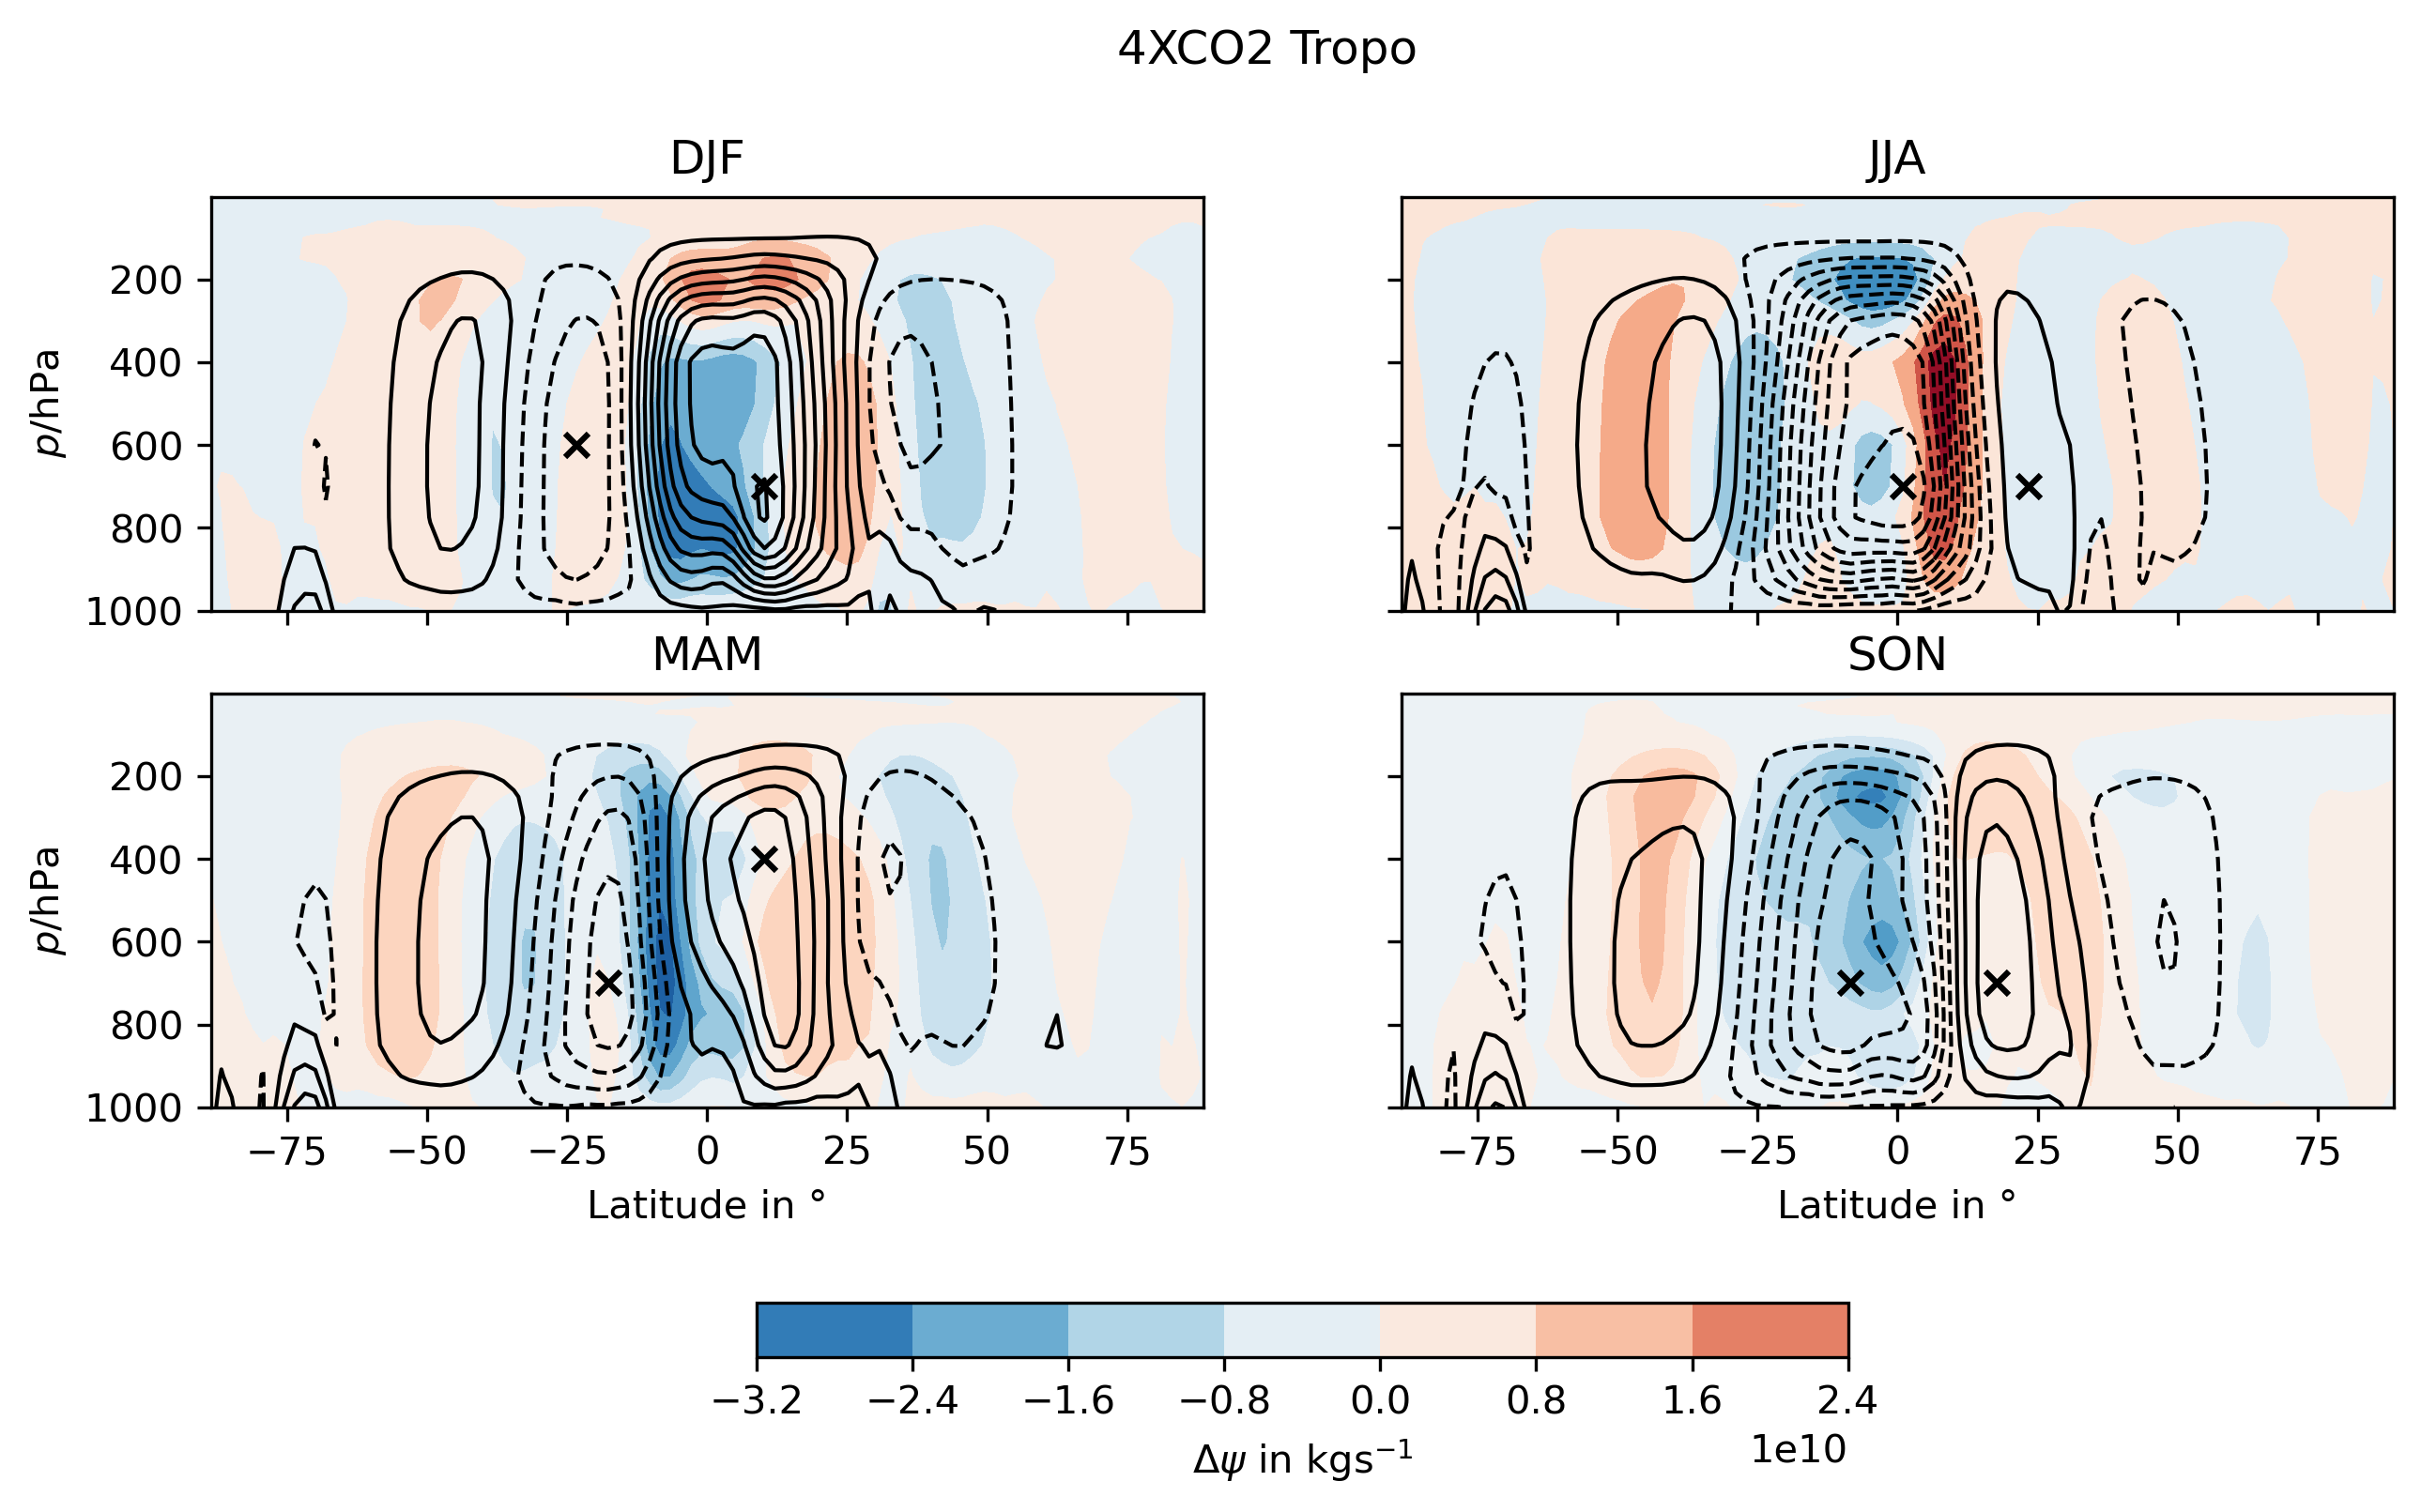
\includegraphics[width=\textwidth]{figures/tropo_seasonal.png}
    \end{figure}
\end{frame}

% \begin{frame}
%     \frametitle{Held \& Hou theory}
%     \begin{figure}
%         \centering
%         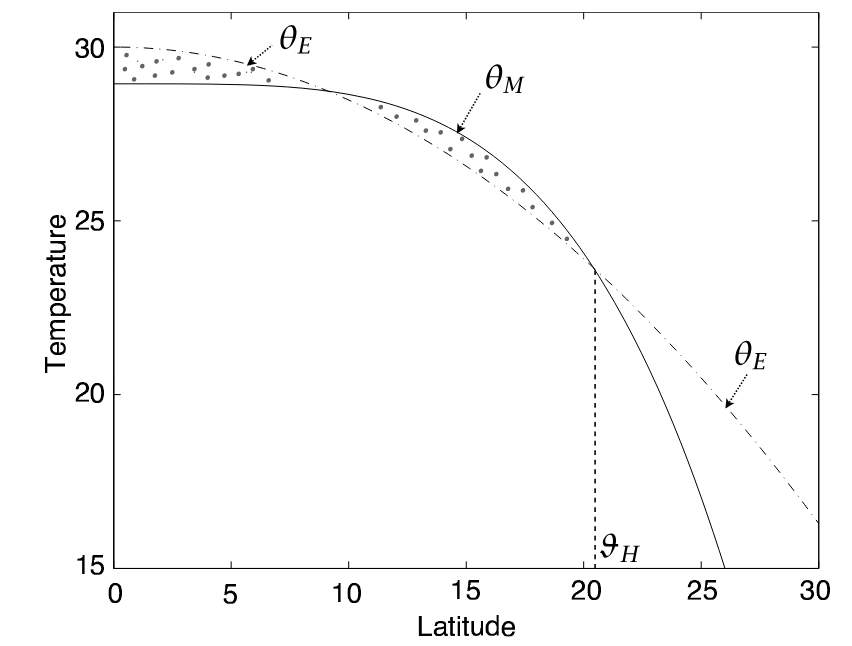
\includegraphics[scale=0.6]{figures/temperature_vallis.png}
%         \caption{\cite{Vallis2017}}
%     \end{figure}
% \end{frame}

% \begin{frame}
%     \frametitle{Axisymmetric scalings}
%     \begin{block}{Width and extent of the HC \cite{HeldHou1980}}  
%     \begin{align}
%         \Phi_H\propto&\left(H\Delta_h\right)^{1/2}\\
%         \psi_\mathrm{max} \propto & \frac{(H\Delta_h)^{5/2}}{\Delta_v}
%     \end{align}
%     \end{block}
%     \begin{itemize}
%         \item global warming response: increase in vertical stability,
%         decrease in meridional temperature contrast, increase in tropopause height
%         \item 
%     \end{itemize}
% \end{frame}





% \begin{frame}
%     \frametitle{H\&H model cannot explain this response}
% \begin{columns}
% \begin{column}{0.3\textwidth}  %%<--- here
 
% \begin{align*}
%     \Phi_H\propto&\left(H\Delta_h\right)^{1/2}\\
%     \psi_\mathrm{max} \propto & \frac{(H\Delta_h)^{5/2}}{\Delta_v}
% \end{align*}

% \end{column}
% \begin{column}{0.58\textwidth}
%     \begin{block}{Forcing response \cite{DAgostino2017}}
%         \begin{itemize}
%             \item Tropopause height $H$ \textbf{increases}
%             \item Meridional temperature gradient $\Delta_h$ \textbf{decreases}
%             \item Vertical stability $\Delta_v$ \textbf{increases} 
%         \end{itemize}
        
%     \end{block}
    
% \end{column}
% \end{columns}
% \end{frame}






% \begin{frame}
%     \frametitle{Zonally averaged circulation}
%     \begin{figure}
%         \centering
%         
\includegraphics[width=\textwidth]{figures/streamfunc.png} %TODO
%     \end{figure}
% \end{frame}

% \begin{frame}
%   \frametitle{Changes in Hadley circulation}
% \begin{table}[]
%     \centering
%     \begin{tabular}{cc|ccc}
%         & PI Control &Uniform & Tropo & Strato \\ \toprule
%         $\psi_\mathrm{max, NH}$& $7.63\cdot10^{10}\;\unit{\kg\s^{-1}}$ & $-0.6\%$ & $4.6\%$& $-7.8\%$\\
%         $\psi_\mathrm{max, SH}$&$-9.66\cdot10^{10}\;\unit{\kg\s^{-1}}$ & $-1.1\%$ & $5.6\%$ & $-6.1\%$\\ 
%         $\Phi_\mathrm{H, NH}$ & $28.85\unit{\degree}$ & $1.35\unit{\degree}$& $0.61\unit{\degree}$ &$0.70\unit{\degree}$\\
%         $\Phi_\mathrm{H, SH}$ &$-30.19\unit{\degree}$ & $-1.46\unit{\degree}$& $-0.93\unit{\degree}$ &$-0.52\unit{\degree}$\\
%     \end{tabular}
%     \label{tab:placeholder}
% \end{table}
% \end{frame}




% \begin{frame}
%     \frametitle{Baroclinic instability and eddy momentum flux}
%     \begin{block}{Baroclinic instability}
%         \begin{align}
%             \theta_C \sim& \left(\frac{NH}{2\Omega a}\right)^{1/2}\\
%         \end{align}
%     \end{block}
%     \begin{block}{Eddy momentum flux}
%         \begin{equation}
%             \psi(1-Ro)\approx \frac{S}{f}
%         \end{equation}
%         \begin{itemize}
%             \item $\mathrm{Ro}\approx 1$: Axisymmetric limit
%             \item $\mathrm{Ro}\approx 1$: Eddy momentum flux dominate
%         \end{itemize}
%     \end{block}
% \end{frame}

\begin{frame}
    \frametitle{More frameworks explaining HC dynamics}
    \begin{itemize}
        % \item Regions of baroclinic instability \cite{phillips1954}
        % \item Eddy momentum and heat flux \cite{WalkerSchneider2006}
        \item Weakening of the overall tropical circulation \cite{VecchiSoden2007}
        \item Energy budget constraints and GMS \cite{ChouChen2010}
    \end{itemize}
\end{frame}

\begin{frame}
    \frametitle{Summary}
    \begin{alertblock}{Research gap}
        We have found the annual mean HC to strengthen under tropospheric CO$_2$ forcing
        while weakening with stratospheric CO$_2$ forcing.
    \end{alertblock}
    \begin{block}{Thesis approach}
        Simplified, axisymmetric frameworks (Held\&Hou) cannot explain this response.
        Indirect thermodynamical drivers will be investigated in a next step.
    \end{block}
    \vfill
    \begin{center}
    \textbf{Thank you for your attention! Do you have any questions?}
    \end{center} 
\end{frame}



% \begin{frame}
%     \frametitle{Workplan}
%     \begin{itemize}
%         \item Apply H\&H scalings to all cases
%         \item Explore different drivers of the HC (e.g., eddy momentum flux)
%         \item Check on different seasonal configurations
%         \item ...
%         \item Thesis submission in October
%     \end{itemize}
%     \vfill
%     \begin{center}
%     \textbf{Thank you for your attention! Do you have any questions?}    
% \end{center}
% \end{frame}

\begin{frame}[allowframebreaks]
    \frametitle{References}
    \bibliography{literature}

\end{frame}

\backupbegin

\begin{frame}
    \frametitle{Is the decomposition valid?}
    \begin{figure}
        \centering
        
\includegraphics[width=\textheight]{figures/non_lin.png}
    \end{figure}
\end{frame}

\begin{frame}
    \frametitle{}
    \begin{figure}
        \centering
        
\includegraphics[width=\textwidth]{figures/scatter_NH.png}
    \end{figure}
\end{frame}

\begin{frame}
    \frametitle{}
    \begin{figure}
        \centering
        
\includegraphics[width=\textwidth]{figures/changes_parameters.png}
    \end{figure}
\end{frame}

\begin{frame}
    \frametitle{}
    \begin{figure}
        \centering
        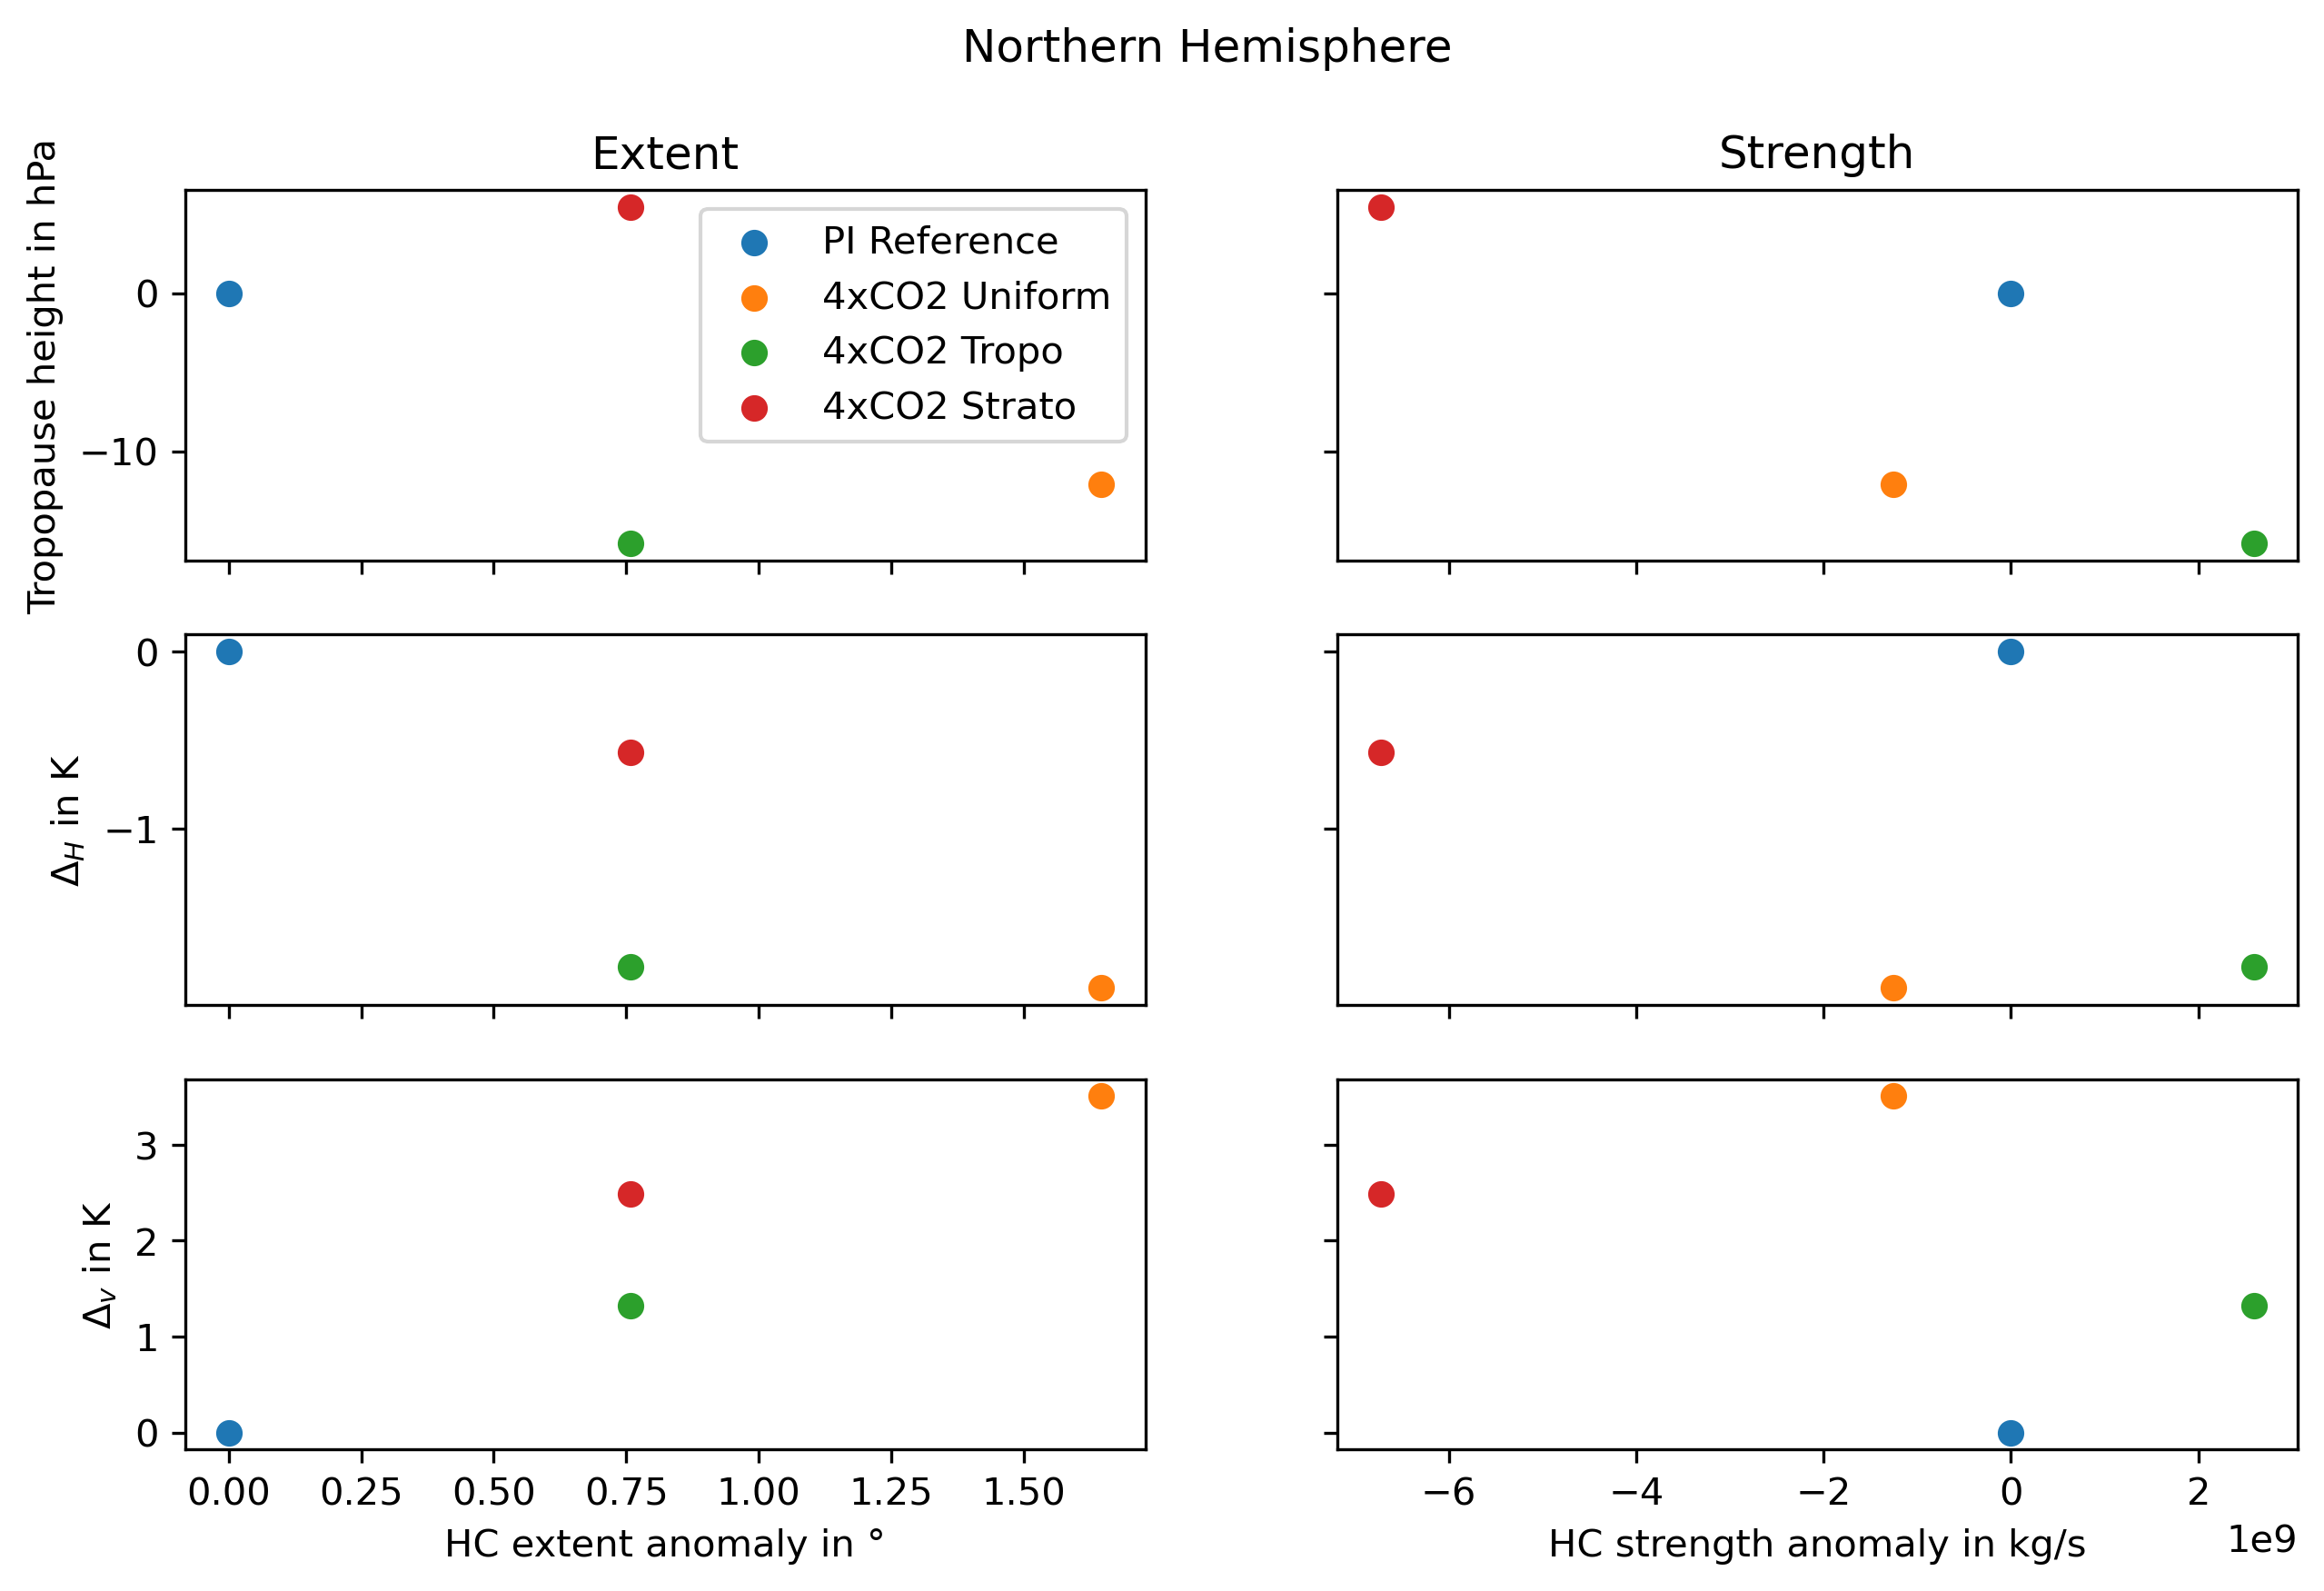
\includegraphics[width=\textwidth]{figures/changes_parameters_NH.png}
    \end{figure}
\end{frame}

\begin{frame}
    \frametitle{}
    \begin{figure}
        \centering
        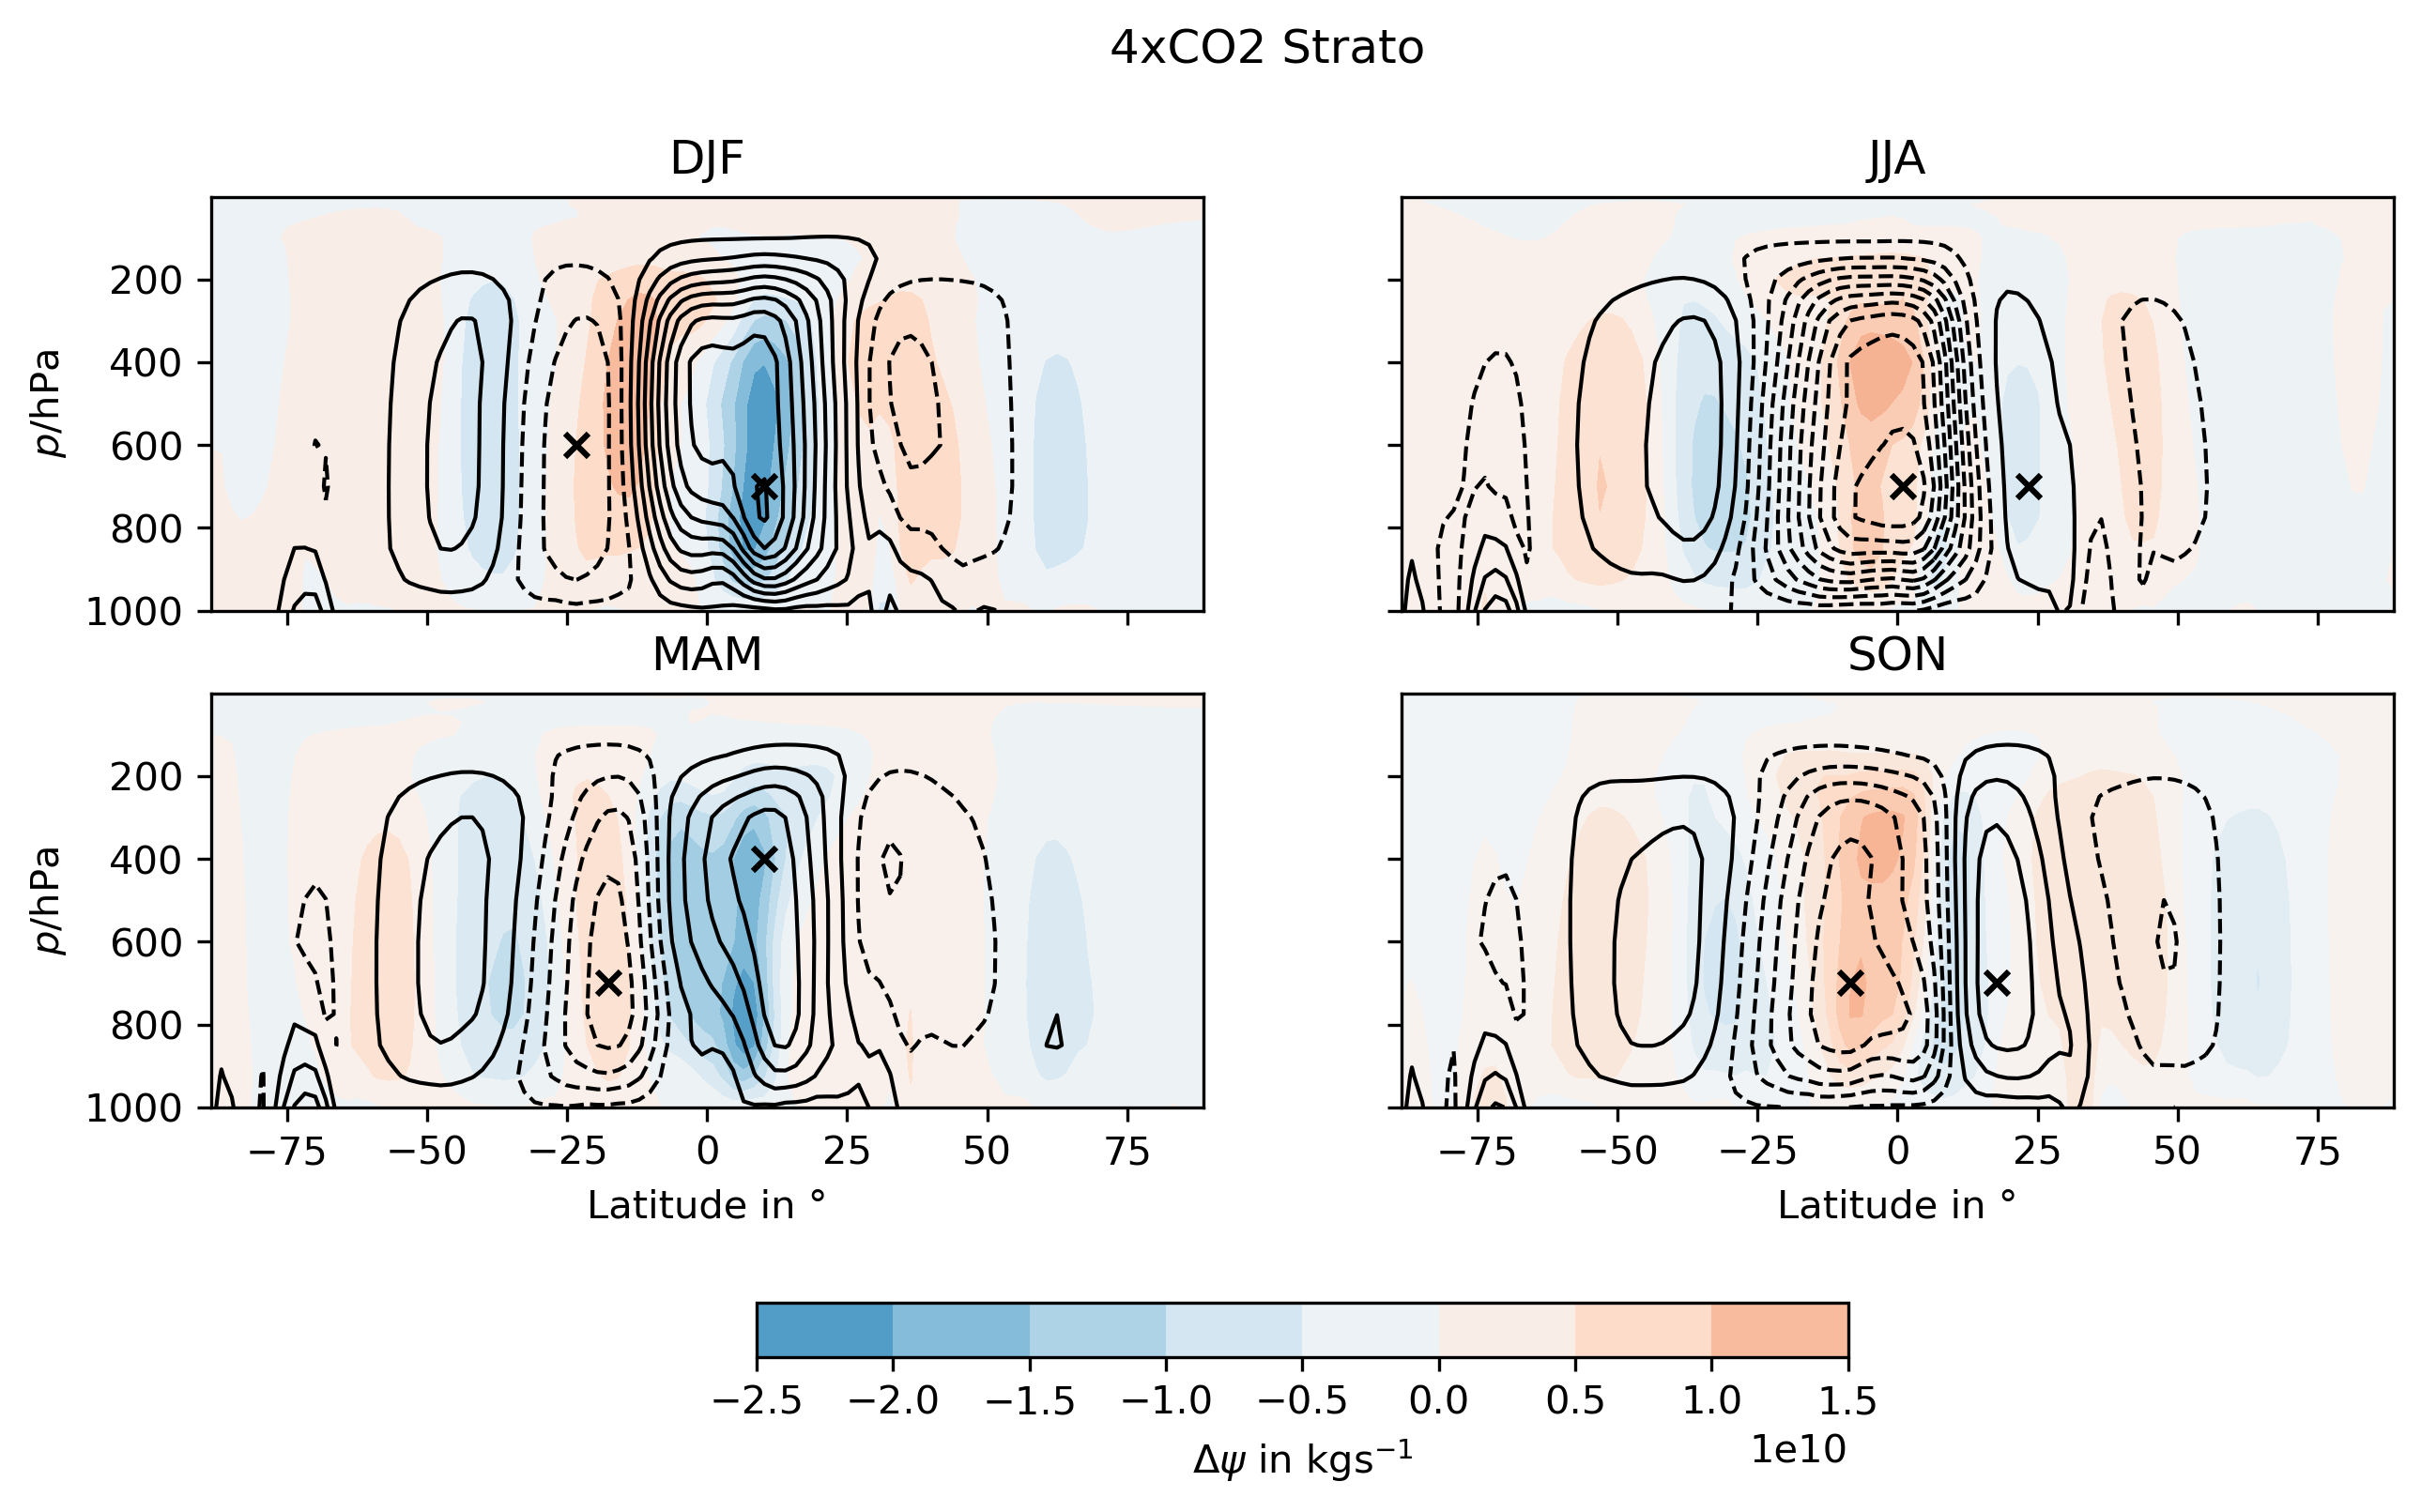
\includegraphics[width=\textwidth]{figures/strato_seasonal.png}
    \end{figure}
\end{frame}

\begin{frame}
    \frametitle{}
    \begin{figure}
        \centering
        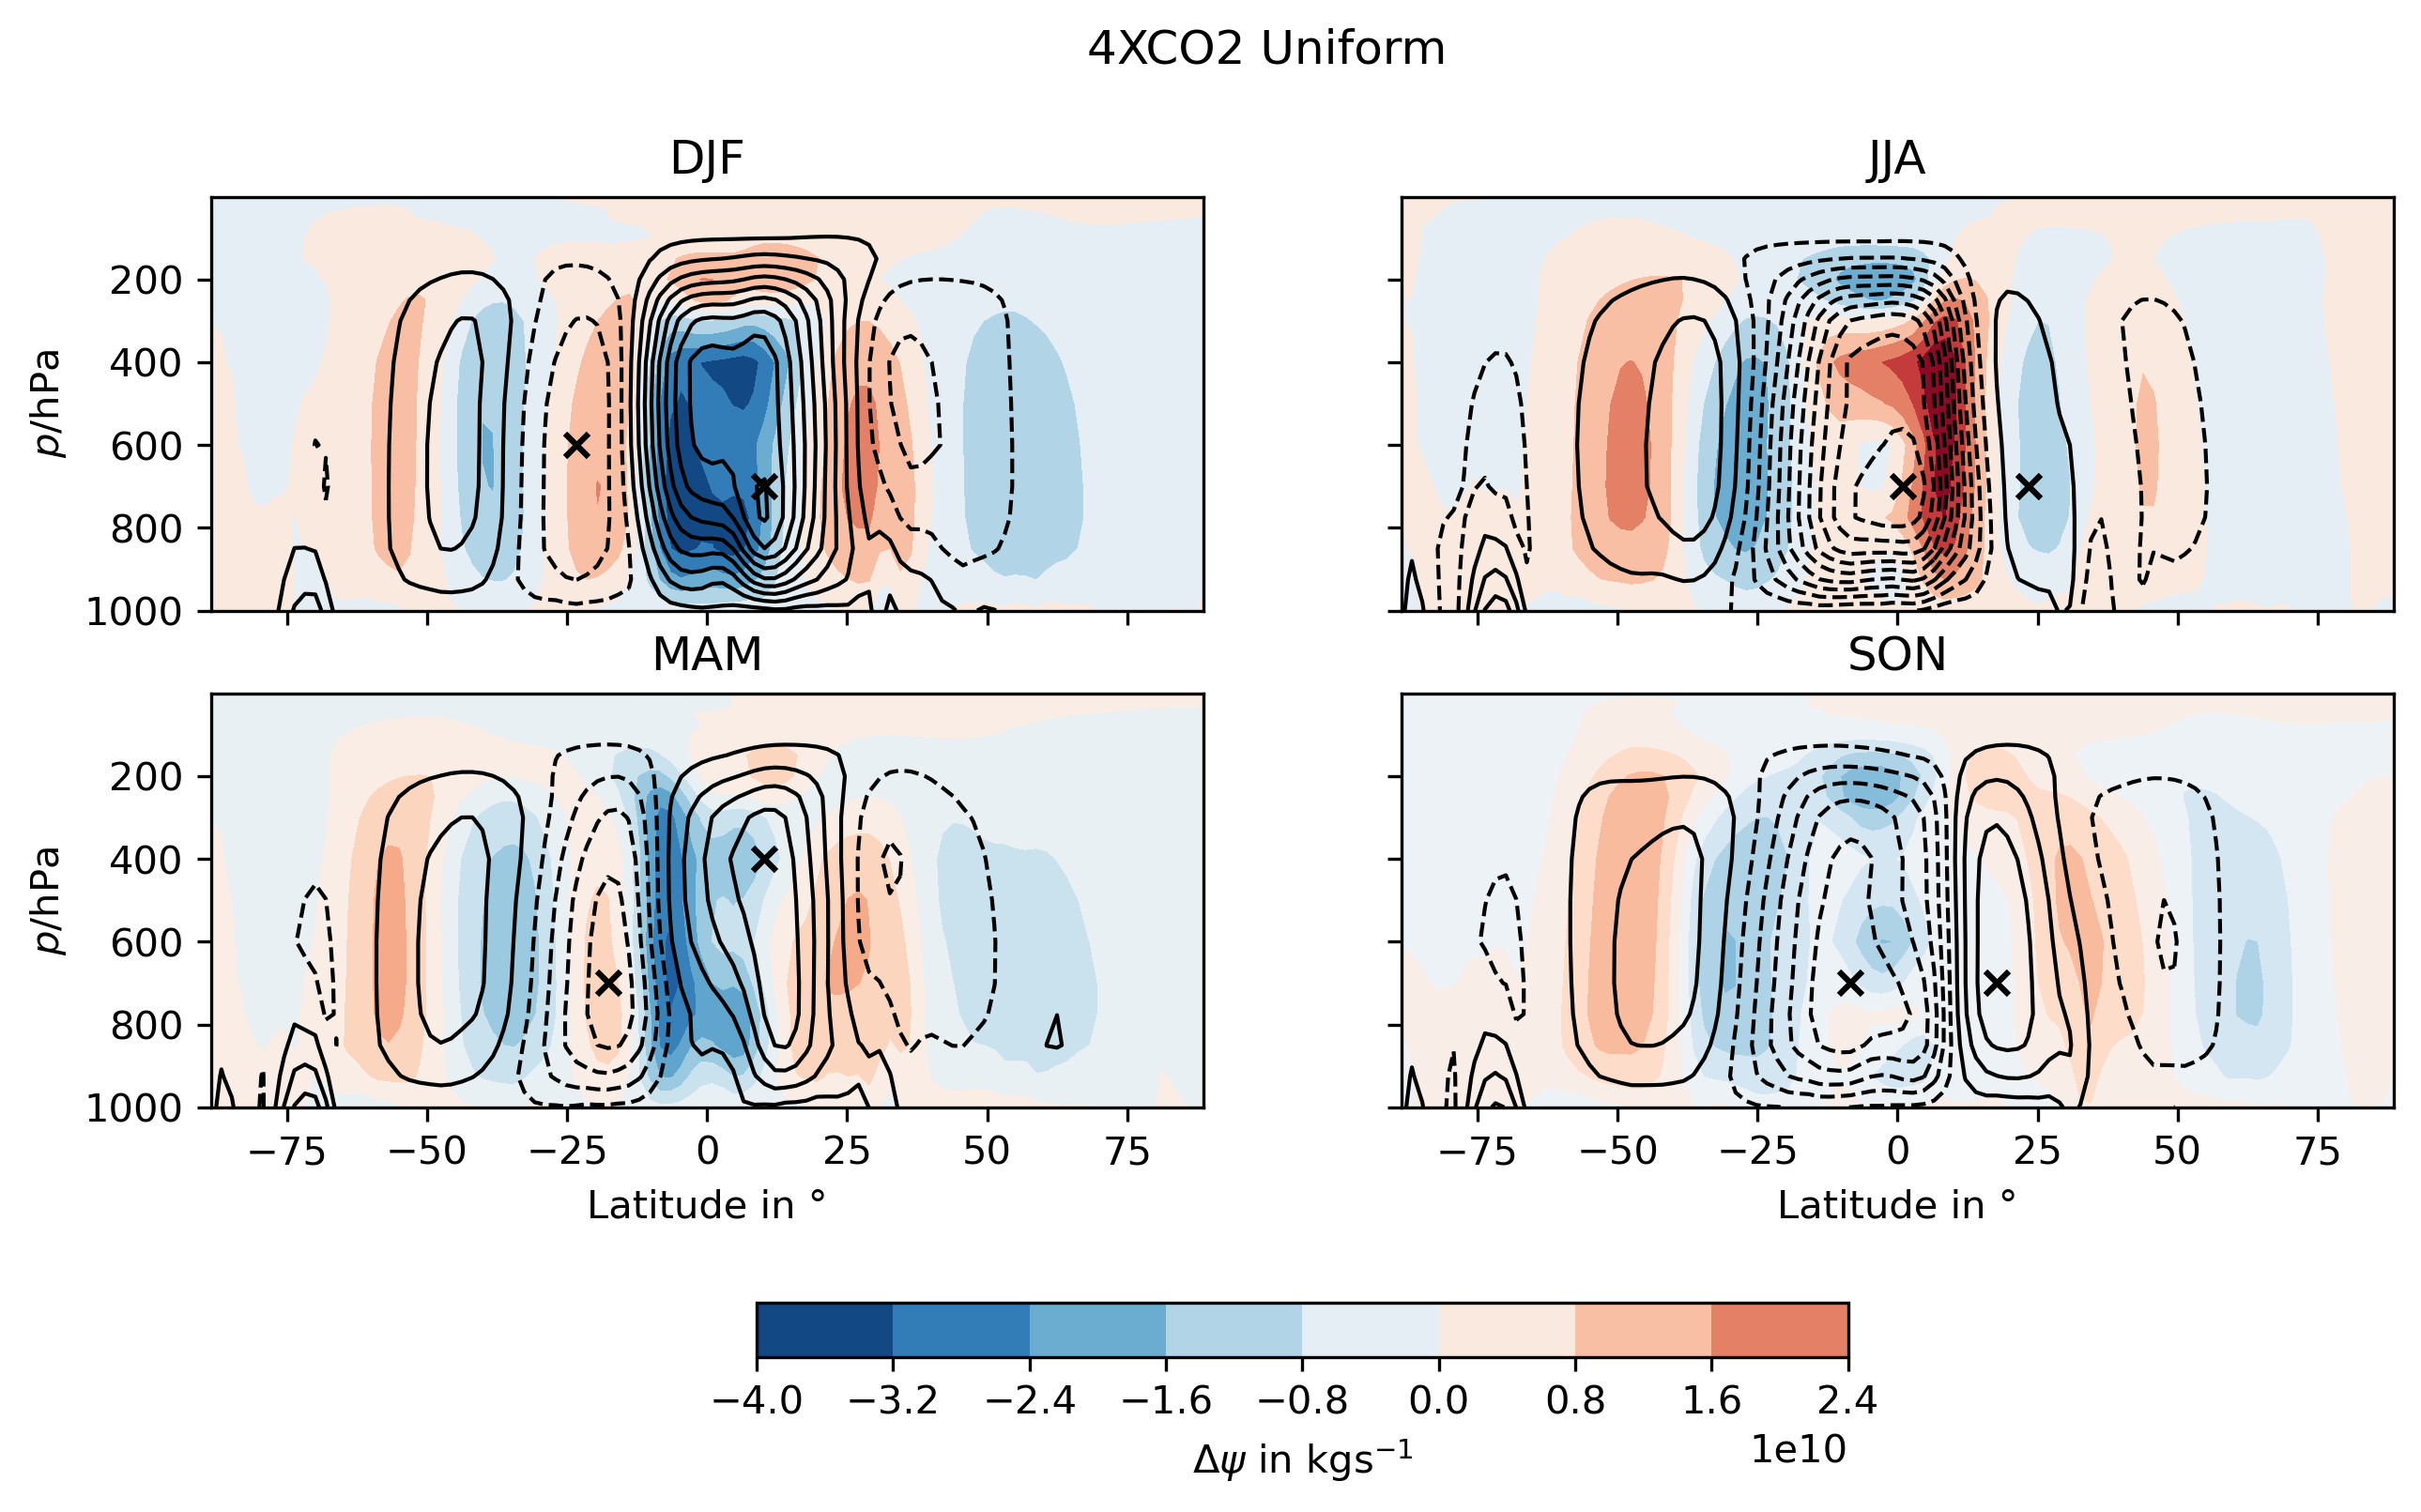
\includegraphics[width=\textwidth]{figures/uniform_seasonal.png}
    \end{figure}
\end{frame}



\backupend
\end{document}
